%
% File: chap01.tex
% Author: Victor F. Brena-Medina
% Description: Introduction chapter where the biology goes.
%
\let\textcircled=\pgftextcircled
\chapter{Anatomy of an Android App}
\label{chap:anatomyOfAnAndroidApp}
\subsection{Application}

\initial{N}ext an app has to be chosen and it has to be an app that has the .apk extension, The app chosen is the Uber app version 3.126.0, which when downloaded, we obtain a com.ubercab-3.126.0-www.APK4Fun.com.apk file.
The procedure that follows is to unzip de .apk and examine the contents, executing unzip command yields the following.

\begin{commandshell}
unzip com.ubercab-3.126.0-www.APK4Fun.com.apk
inflating: AndroidManifest.xml     
   creating: assets/
  inflating: assets/crashlytics-build.properties  
   creating: assets/fonts/
  inflating: assets/fonts/ClanPro-Book.otf  
  inflating: assets/fonts/ClanPro-Medium.otf  
  inflating: assets/fonts/ClanPro-NarrBook.otf  
  inflating: assets/fonts/ClanPro-NarrMedium.otf  
  inflating: assets/fonts/ClanPro-NarrNews.otf  
  inflating: assets/fonts/ClanPro-News.otf  
...
\end{commandshell}
\begin{commandshell}
apktool d com.ubercab-3.126.0-www.APK4Fun.com.apk 
Picked up _JAVA_OPTIONS:   -Dawt.useSystemAAFontSettings=gasp
I: Using Apktool 2.2.1 on com.ubercab-3.126.0-www.APK4Fun.com.apk
I: Loading resource table...
I: Decoding AndroidManifest.xml with resources...
I: Loading resource table from file: /home/danielftapiar/.local/share/apktool/framework/1.apk
I: Regular manifest package...
I: Decoding file-resources...
I: Decoding values */* XMLs...
I: Baksmaling classes.dex...
I: Baksmaling classes2.dex...
I: Baksmaling classes3.dex...
I: Baksmaling classes4.dex...
I: Copying assets and libs...
I: Copying unknown files...
I: Copying original files...

\end{commandshell}

\subsection{Directory Listing}
\begin{tikzpicture}[%
    scale=.7,
    grow via three points={one child at (0.5,-0.65) and
    two children at (0.5,-0.65) and (0.5,-1.1)},
    edge from parent path={(\tikzparentnode.south) |- (\tikzchildnode.west)}]
  \node [root] {unzipped}
    child { node [selected] {assets}
      child { node { crashlytics-build.properties}}
      child { node [selected] {fonts}}
      child { node [selected] {geofences}}
      child { node [selected] {geojson}}
      child { node [selected] {licenses}}
      child { node [selected] {splash}}
    }       
    child { node at (0,-3.5) [selected] {res}
      child { node [selected] {animator}}
      child { node [selected] {menu}}
      child { node [selected] {layout}}
      child { node [selected] {...}}
    }
    child { node at (0,-5.9) [selected] {lib}
      child { node [selected] {armeabi-v7a}}
    }
    child { node at (0,-7.0) [selected] {META-INF}
      child { node {CERT.RSA}}
      child { node {CERT.SF}}
      child { node {MANIFEST.MF}}
      child { node [selected] {services}}
    }
    child { node at (0,-9.5) {AndroidManifest.xml}}
    child { node at (0,-9.5) {build-data.properties}}
    child { node at (0,-9.5) {classes2.dex}}
    child { node at (0,-9.5) {classes3.dex}}
    child { node at (0,-9.5) {classes4.dex}}
    child { node at (0,-9.5) {classes.dex}}
    child { node at (0,-9.5) {resources.arsc}}
    ;
\end{tikzpicture}

As it can be seen the .apk format is really just a zipped archive with the binaries compiled, a breakdown of these directories is as follows.

\subsection{classes.dex}
Contains compiled application code, transformed into Dex bytecode. You might see more than one DEX file in your APK if you are using multidex to overcome the 65536 method limit. Beginning with Android 5.0 which introduced the ART runtime, these are compiled into OAT files by the ahead-of-time compiler at install time and put on the device’s data partition.
\subsection{res/}

This folder contains most XML resources (e.g. layouts) and drawables (e.g. PNG, JPEG) in folders with various qualifiers, like -mdpi and -hdpi for densities, -sw600dp or -large for screen sizes and -en, -de, -pl for languages. Please note that any XML files in res/ have been transformed into a more compact, binary representation at compile time, so you won’t be able to open them with a text editor from inside the APK.

\subsection{resources.arsc}

Some resources and identifiers are compiled and flattened into this file. It’s normally stored in the APK without compression for faster access during runtime. Compressing this file manually might seem like an easy win, but is actually not a good idea for at least two reasons. One, Play Store compresses any data for transfer anyway and two, having the file compressed inside the APK would waste system resources (RAM) and performance (especially app startup time).

\subsection{AndroidManifest.xml}

Similar to other XML resources, your application Manifest is transformed during compilation into a binary format. Play Store uses certain information contained in the AndroidManifest to decide if an APK can be installed on a device, checking against allowed densities or screen sizes and available hardware and features (such as a touchscreen). If you want to inspect those Manifest entries after compilation, you can use the aapt tool from the Android SDK:

\begin{minted}
[bgcolor = lightGrey]
{bash}
  $ apt dump badging your_app.apk
\end{minted}

\end{document}
\subsection{libs/}

\subsection{assets/}
This folder is used for any file assets that will not be used as Android-type resources. Most commonly this will be font files or game data, like levels and textures, as well as any other application data that you want to open directly as a file stream.
\subsection{META-INF/}
This folder is present in signed APKs and contains a list of all files in the APK with their signatures. The way signing in Android works currently is that it verifies the signatures against uncompressed file contents from the archive, one by one.
This has some interesting consequences. Because every entry in a ZIP file is stored separately, this means that you can change individual files’ compression level without re-signing. The signature verification will fail however if you remove any file from the archive after it is signed.
One more thing to note about how a signed APK is created is that the zipalign tool is used as the last stage of the build. If you change the contents of the archive by hand, normally you will have to re-sign, then zipalign before uploading the APK to the Play Store.

% \label{subsec:subsec01}

% Begins a subsection.

% %A figures matrix.
% \begin{figure}[t!]
% \centering
% \begin{minipage}{3.3cm}
%     \centering
%     \subtop[]{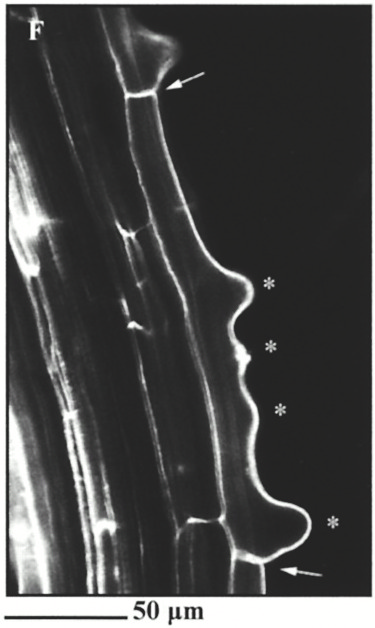
\includegraphics[height=0.28\textheight]{fig01/Nswellings}\label{sf:multiRH02a}}
% \end{minipage}
% \hspace{0.5cm}
% \begin{minipage}{3.3cm}
%     \centering
%     \subtop[]{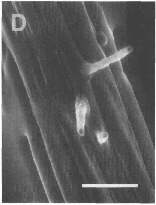
\includegraphics[height=0.27\textheight]{fig01/Mswellings}\label{sf:multiRH02b}}
% \end{minipage}
% \hspace{1.3cm}
% \begin{minipage}{3.3cm}
%     \centering
%     \subtop[]{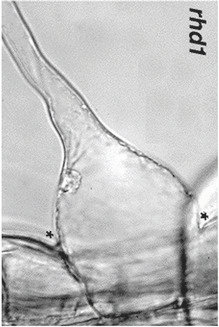
\includegraphics[height=0.27\textheight]{fig01/rhd1}\label{sf:multiRH02c}}
% \end{minipage}
% \\ \vspace{0.1cm}
% \begin{minipage}{10cm}
%     \centering
%     \subtop[]{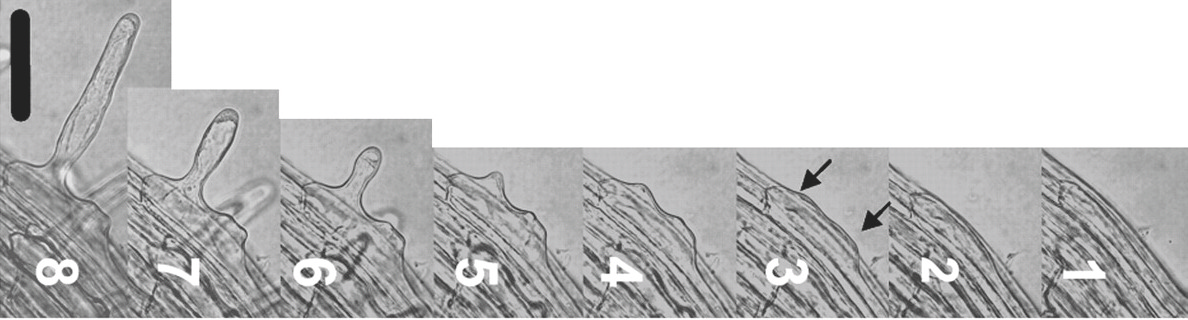
\includegraphics[height=0.145\textheight]{fig01/mutantrhd6}\label{sf:multiRH02d}}
% \end{minipage}
% \\ \vspace{0.1cm}
% \begin{minipage}{10cm}
%     \centering
%     \subtop[]{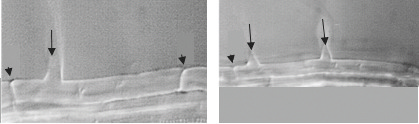
\includegraphics[height=0.16\textheight]{fig01/auxab}\label{sf:multiRH02e}}
% \end{minipage}
% \mycaption[Hair-forming mutant cells.]{(a) A mutant RH cell. Asterisks show multiple sites of RH initiation in a single root hair cell (indicated by the arrows). Figure reproduced from \cite{rigas01}. (b)~Hair-forming cell with three RH initiation locations. The bar represents $50\mu m$. Figure reproduced from \cite{massuci01}. (c) Large bump in mutant {\itshape rhd1}. Figure reproduced from \cite{griersonRH}. (d) Mutant overexpressing gene {\itshape ROP2}; from right-hand to left-hand, numbers indicate progressive snapshots at different times. RH initiation sites are indicated by the arrows. The bar represents $75\mu m$. Figure reproduced from~\cite{mjones01}. (e)~Mutants affected by auxin. On the left-hand side, RH site is farther away from the apical end (left arrow cap); on the right-hand side, multiple RH locations (arrows). Figure reproduced from~\cite{payne01}.}
% \label{fig:multiRH02}
% \end{figure}

% % A single figure
% \begin{figure}[t!]
% 	\centering
% 	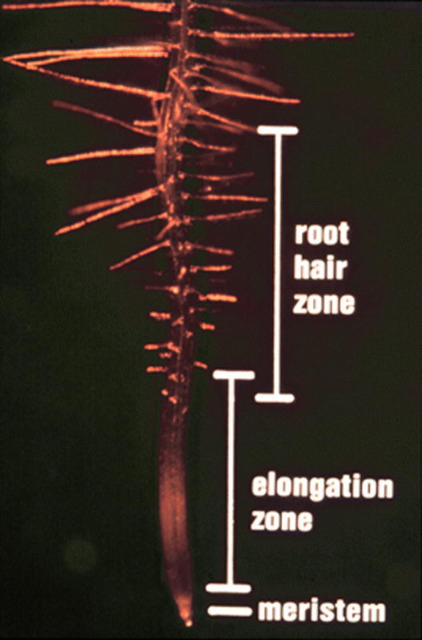
\includegraphics[height=0.35\textheight]{fig01/devepzones}
% 	\mycaption[Developmental zones of an Arabidopsis root.]{Developmental zones of an Arabidopsis root. Figure reproduced from \cite{griersonRH}.}
% 	\label{fig:RHP02}
% \end{figure}

%=========================================================